\documentclass[11pt,a4paper]{article}
\newcommand{\tipodoc}{Reporte técnico}
% Preámbulo común para los documentos de apoyo de GreenSense IoT
% Antes de % Preámbulo común para los documentos de apoyo de GreenSense IoT
% Antes de % Preámbulo común para los documentos de apoyo de GreenSense IoT
% Antes de \input{preambulo} se define \newcommand{\tipodoc}{...}

\usepackage{fontspec}
\usepackage[spanish,es-tabla,es-nodecimaldot,es-noshorthands]{babel}
\setmainfont{TeX Gyre Termes}
\setsansfont{TeX Gyre Heros}
\usepackage{microtype}

\hyphenpenalty=10000
\exhyphenpenalty=10000
\emergencystretch=3em

\usepackage[top=2.5cm,bottom=2.5cm,left=2.5cm,right=2.5cm,headheight=15pt]{geometry}
\usepackage{setspace}
\setstretch{1.15}
\setlength{\parskip}{0.45em}
\setlength{\parindent}{0pt}

\usepackage[table]{xcolor}
\definecolor{upqazul}{HTML}{002D72}
\definecolor{upqrojo}{HTML}{BA0C2F}
\definecolor{grisborde}{HTML}{8C8C8C}
\definecolor{grisfondo}{HTML}{F2F2F2}

\usepackage{array}
\usepackage{tabularx}
\usepackage{booktabs}
\usepackage{float}
\usepackage{enumitem}
\usepackage{caption}
\usepackage{needspace}
\usepackage[most]{tcolorbox}

\captionsetup{font={small},labelfont={bf,color=upqazul},labelsep=period,skip=6pt}
\setlist{itemsep=0.2em,topsep=0.3em,leftmargin=1.6em}
\setlist[itemize]{label={\color{upqazul}\small$\bullet$}}
\setlist[enumerate]{label={\color{upqazul}\arabic*.}}
\newcolumntype{L}{>{\raggedright\arraybackslash}X}
\newcolumntype{P}[1]{>{\raggedright\arraybackslash}p{#1}}
\renewcommand{\arraystretch}{1.25}

\usepackage{titlesec}
\titleformat{\section}
  {\needspace{8\baselineskip}\normalfont\Large\bfseries\color{upqazul}}
  {\thesection.}{0.6em}{}[{\color{upqrojo}\titlerule[0.8pt]}]
\titleformat{\subsection}
  {\needspace{5\baselineskip}\normalfont\large\bfseries\color{upqazul}}
  {\thesubsection}{0.6em}{}
\titleformat{\subsubsection}
  {\needspace{4\baselineskip}\normalfont\normalsize\bfseries\color{upqazul}}
  {}{0em}{}
\titlespacing*{\section}{0pt}{1.4em}{0.8em}
\titlespacing*{\subsection}{0pt}{1.1em}{0.4em}
\titlespacing*{\subsubsection}{0pt}{0.9em}{0.3em}

\usepackage{lastpage}
\usepackage{fancyhdr}
\pagestyle{fancy}
\fancyhf{}
\fancyhead[L]{\small\color{upqazul}Proyecto HPC · Detección de bordes en Kubernetes}
\fancyhead[R]{\small\color{upqazul}\tipodoc}
\fancyfoot[C]{\small Página \thepage\ de \pageref{LastPage}}
\renewcommand{\headrule}{{\color{upqrojo}\hrule height 0.6pt}}
\renewcommand{\footrulewidth}{0pt}
\fancypagestyle{plain}{\fancyhf{}\renewcommand{\headrule}{}\fancyfoot[C]{\small Página \thepage\ de \pageref{LastPage}}}

\usepackage{tocloft}
\renewcommand{\cftsecfont}{\bfseries\color{upqazul}}
\renewcommand{\cftsecpagefont}{\bfseries\color{upqazul}}
\renewcommand{\cftsecleader}{\cftdotfill{\cftdotsep}}
\setlength{\cftbeforesecskip}{0.45em}

\usepackage[hidelinks]{hyperref}
\urlstyle{same}

% Recuadros
\newtcolorbox{recuadro}[1][]{enhanced,colback=grisfondo,colframe=grisfondo,
  boxrule=0pt,arc=2pt,left=8pt,right=8pt,top=6pt,bottom=6pt,#1}
\newtcolorbox{recuadroazul}[1]{enhanced,colback=white,colframe=upqazul,
  boxrule=0.8pt,arc=2pt,left=8pt,right=8pt,top=6pt,bottom=6pt,
  title={\bfseries #1},coltitle=white,colbacktitle=upqazul,fonttitle=\small}

% Pregunta frecuente: \pregunta{Área}{Pregunta}{Respuesta}
\newcounter{numpregunta}
\newcommand{\pregunta}[3]{%
  \stepcounter{numpregunta}%
  \needspace{5\baselineskip}%
  \textbf{\color{upqazul}\thenumpregunta. #2}\hfill{\small\color{grisborde}#1}\par\nopagebreak
  #3\par\medskip}
 se define \newcommand{\tipodoc}{...}

\usepackage{fontspec}
\usepackage[spanish,es-tabla,es-nodecimaldot,es-noshorthands]{babel}
\setmainfont{TeX Gyre Termes}
\setsansfont{TeX Gyre Heros}
\usepackage{microtype}

\hyphenpenalty=10000
\exhyphenpenalty=10000
\emergencystretch=3em

\usepackage[top=2.5cm,bottom=2.5cm,left=2.5cm,right=2.5cm,headheight=15pt]{geometry}
\usepackage{setspace}
\setstretch{1.15}
\setlength{\parskip}{0.45em}
\setlength{\parindent}{0pt}

\usepackage[table]{xcolor}
\definecolor{upqazul}{HTML}{002D72}
\definecolor{upqrojo}{HTML}{BA0C2F}
\definecolor{grisborde}{HTML}{8C8C8C}
\definecolor{grisfondo}{HTML}{F2F2F2}

\usepackage{array}
\usepackage{tabularx}
\usepackage{booktabs}
\usepackage{float}
\usepackage{enumitem}
\usepackage{caption}
\usepackage{needspace}
\usepackage[most]{tcolorbox}

\captionsetup{font={small},labelfont={bf,color=upqazul},labelsep=period,skip=6pt}
\setlist{itemsep=0.2em,topsep=0.3em,leftmargin=1.6em}
\setlist[itemize]{label={\color{upqazul}\small$\bullet$}}
\setlist[enumerate]{label={\color{upqazul}\arabic*.}}
\newcolumntype{L}{>{\raggedright\arraybackslash}X}
\newcolumntype{P}[1]{>{\raggedright\arraybackslash}p{#1}}
\renewcommand{\arraystretch}{1.25}

\usepackage{titlesec}
\titleformat{\section}
  {\needspace{8\baselineskip}\normalfont\Large\bfseries\color{upqazul}}
  {\thesection.}{0.6em}{}[{\color{upqrojo}\titlerule[0.8pt]}]
\titleformat{\subsection}
  {\needspace{5\baselineskip}\normalfont\large\bfseries\color{upqazul}}
  {\thesubsection}{0.6em}{}
\titleformat{\subsubsection}
  {\needspace{4\baselineskip}\normalfont\normalsize\bfseries\color{upqazul}}
  {}{0em}{}
\titlespacing*{\section}{0pt}{1.4em}{0.8em}
\titlespacing*{\subsection}{0pt}{1.1em}{0.4em}
\titlespacing*{\subsubsection}{0pt}{0.9em}{0.3em}

\usepackage{lastpage}
\usepackage{fancyhdr}
\pagestyle{fancy}
\fancyhf{}
\fancyhead[L]{\small\color{upqazul}Proyecto HPC · Detección de bordes en Kubernetes}
\fancyhead[R]{\small\color{upqazul}\tipodoc}
\fancyfoot[C]{\small Página \thepage\ de \pageref{LastPage}}
\renewcommand{\headrule}{{\color{upqrojo}\hrule height 0.6pt}}
\renewcommand{\footrulewidth}{0pt}
\fancypagestyle{plain}{\fancyhf{}\renewcommand{\headrule}{}\fancyfoot[C]{\small Página \thepage\ de \pageref{LastPage}}}

\usepackage{tocloft}
\renewcommand{\cftsecfont}{\bfseries\color{upqazul}}
\renewcommand{\cftsecpagefont}{\bfseries\color{upqazul}}
\renewcommand{\cftsecleader}{\cftdotfill{\cftdotsep}}
\setlength{\cftbeforesecskip}{0.45em}

\usepackage[hidelinks]{hyperref}
\urlstyle{same}

% Recuadros
\newtcolorbox{recuadro}[1][]{enhanced,colback=grisfondo,colframe=grisfondo,
  boxrule=0pt,arc=2pt,left=8pt,right=8pt,top=6pt,bottom=6pt,#1}
\newtcolorbox{recuadroazul}[1]{enhanced,colback=white,colframe=upqazul,
  boxrule=0.8pt,arc=2pt,left=8pt,right=8pt,top=6pt,bottom=6pt,
  title={\bfseries #1},coltitle=white,colbacktitle=upqazul,fonttitle=\small}

% Pregunta frecuente: \pregunta{Área}{Pregunta}{Respuesta}
\newcounter{numpregunta}
\newcommand{\pregunta}[3]{%
  \stepcounter{numpregunta}%
  \needspace{5\baselineskip}%
  \textbf{\color{upqazul}\thenumpregunta. #2}\hfill{\small\color{grisborde}#1}\par\nopagebreak
  #3\par\medskip}
 se define \newcommand{\tipodoc}{...}

\usepackage{fontspec}
\usepackage[spanish,es-tabla,es-nodecimaldot,es-noshorthands]{babel}
\setmainfont{TeX Gyre Termes}
\setsansfont{TeX Gyre Heros}
\usepackage{microtype}

\hyphenpenalty=10000
\exhyphenpenalty=10000
\emergencystretch=3em

\usepackage[top=2.5cm,bottom=2.5cm,left=2.5cm,right=2.5cm,headheight=15pt]{geometry}
\usepackage{setspace}
\setstretch{1.15}
\setlength{\parskip}{0.45em}
\setlength{\parindent}{0pt}

\usepackage[table]{xcolor}
\definecolor{upqazul}{HTML}{002D72}
\definecolor{upqrojo}{HTML}{BA0C2F}
\definecolor{grisborde}{HTML}{8C8C8C}
\definecolor{grisfondo}{HTML}{F2F2F2}

\usepackage{array}
\usepackage{tabularx}
\usepackage{booktabs}
\usepackage{float}
\usepackage{enumitem}
\usepackage{caption}
\usepackage{needspace}
\usepackage[most]{tcolorbox}

\captionsetup{font={small},labelfont={bf,color=upqazul},labelsep=period,skip=6pt}
\setlist{itemsep=0.2em,topsep=0.3em,leftmargin=1.6em}
\setlist[itemize]{label={\color{upqazul}\small$\bullet$}}
\setlist[enumerate]{label={\color{upqazul}\arabic*.}}
\newcolumntype{L}{>{\raggedright\arraybackslash}X}
\newcolumntype{P}[1]{>{\raggedright\arraybackslash}p{#1}}
\renewcommand{\arraystretch}{1.25}

\usepackage{titlesec}
\titleformat{\section}
  {\needspace{8\baselineskip}\normalfont\Large\bfseries\color{upqazul}}
  {\thesection.}{0.6em}{}[{\color{upqrojo}\titlerule[0.8pt]}]
\titleformat{\subsection}
  {\needspace{5\baselineskip}\normalfont\large\bfseries\color{upqazul}}
  {\thesubsection}{0.6em}{}
\titleformat{\subsubsection}
  {\needspace{4\baselineskip}\normalfont\normalsize\bfseries\color{upqazul}}
  {}{0em}{}
\titlespacing*{\section}{0pt}{1.4em}{0.8em}
\titlespacing*{\subsection}{0pt}{1.1em}{0.4em}
\titlespacing*{\subsubsection}{0pt}{0.9em}{0.3em}

\usepackage{lastpage}
\usepackage{fancyhdr}
\pagestyle{fancy}
\fancyhf{}
\fancyhead[L]{\small\color{upqazul}Proyecto HPC · Detección de bordes en Kubernetes}
\fancyhead[R]{\small\color{upqazul}\tipodoc}
\fancyfoot[C]{\small Página \thepage\ de \pageref{LastPage}}
\renewcommand{\headrule}{{\color{upqrojo}\hrule height 0.6pt}}
\renewcommand{\footrulewidth}{0pt}
\fancypagestyle{plain}{\fancyhf{}\renewcommand{\headrule}{}\fancyfoot[C]{\small Página \thepage\ de \pageref{LastPage}}}

\usepackage{tocloft}
\renewcommand{\cftsecfont}{\bfseries\color{upqazul}}
\renewcommand{\cftsecpagefont}{\bfseries\color{upqazul}}
\renewcommand{\cftsecleader}{\cftdotfill{\cftdotsep}}
\setlength{\cftbeforesecskip}{0.45em}

\usepackage[hidelinks]{hyperref}
\urlstyle{same}

% Recuadros
\newtcolorbox{recuadro}[1][]{enhanced,colback=grisfondo,colframe=grisfondo,
  boxrule=0pt,arc=2pt,left=8pt,right=8pt,top=6pt,bottom=6pt,#1}
\newtcolorbox{recuadroazul}[1]{enhanced,colback=white,colframe=upqazul,
  boxrule=0.8pt,arc=2pt,left=8pt,right=8pt,top=6pt,bottom=6pt,
  title={\bfseries #1},coltitle=white,colbacktitle=upqazul,fonttitle=\small}

% Pregunta frecuente: \pregunta{Área}{Pregunta}{Respuesta}
\newcounter{numpregunta}
\newcommand{\pregunta}[3]{%
  \stepcounter{numpregunta}%
  \needspace{5\baselineskip}%
  \textbf{\color{upqazul}\thenumpregunta. #2}\hfill{\small\color{grisborde}#1}\par\nopagebreak
  #3\par\medskip}

\usepackage{graphicx}
\usepackage{amsmath}
\usepackage{xurl}
\setmonofont{DejaVu Sans Mono}[Scale=0.8]
\geometry{top=2.2cm,bottom=2.2cm,left=2.2cm,right=2.2cm}
\setstretch{1.05}
\graphicspath{{../../resultados/}}
\hypersetup{pdftitle={Detección de bordes por lotes con Jobs indexados en Kubernetes}}

\begin{document}

% ---------------------------------------------------------------- Portada
\begin{titlepage}
\thispagestyle{empty}
\centering
{\color{upqazul}\rule{\linewidth}{1.4pt}}\par
\vspace{0.2cm}
{\large\scshape Universidad Politécnica de Querétaro}\par
\vspace{0.1cm}
{\normalsize Ingeniería en Datos e Inteligencia Artificial · Grupo IDIA211}\par
\vspace{0.2cm}
{\color{upqrojo}\rule{\linewidth}{0.6pt}}\par
\vspace{3cm}
{\fontsize{26}{32}\selectfont\bfseries\color{upqazul} Detección de bordes por lotes\\[0.2cm] con Jobs indexados en Kubernetes\par}
\vspace{0.6cm}
{\Large Proyecto de Cómputo de Alto Rendimiento\par}
\vspace{0.3cm}
{\large\itshape Equipo 5 · Dataset Oxford-IIIT Pet\par}
\vfill
\begin{tabular}{l@{\hspace{1.5cm}}l}
Diego Cortes Zermeño & 124048766\\
Irving Nahir Ferrusca Jaimez & 124048614\\
César Iván Ramírez Castañon & 124051715\\
Axel Miguel Quevedo Barrios & 124051378\\
\end{tabular}

\vspace{0.8cm}
\begin{tabular}{@{}r@{\hspace{0.6cm}}l@{}}
\textbf{Materia} & Cómputo de Alto Rendimiento\\
\textbf{Docente} & Javier Moya\\
\textbf{Repositorio} & \url{https://github.com/DiegoZerm/bordes-k8s}\\
\textbf{Fecha} & 26 de noviembre de 2026\\
\end{tabular}

\vspace{0.8cm}
{\color{upqrojo}\rule{\linewidth}{0.6pt}}\par
\end{titlepage}
\setcounter{page}{2}

% ---------------------------------------------------------------- 1
\section{Arquitectura}

Procesamos las \textbf{7,390 fotos} del tar oficial de Oxford-IIIT Pet: 775~MB, de 0.01 a 8~megapíxeles, mediana de 0.17~MP. La tabla del curso dice 7,349 porque ese es el número de fotos con anotación. Cada foto pasa por \emph{escala de grises $\rightarrow$ desenfoque gaussiano ($\sigma = 1.4$) $\rightarrow$ Sobel $\rightarrow$ umbral}. El Sobel está hecho con \emph{slicing} de numpy sobre una imagen de Pillow. Todo corre en \textbf{kind}: un control-plane y 3 workers, que son contenedores de Docker en una laptop con Ryzen~5 3550H (4 núcleos físicos, 8 hilos) y 22~GB de RAM.

\begin{enumerate}
\item \textbf{Datos compartidos.} kind monta la carpeta \texttt{datos/} del repositorio en \texttt{/data} de los 3 workers, y el Job la usa con un volumen \texttt{hostPath}. Las fotos están en \texttt{/data/entrada} y cada corrida escribe en \texttt{/data/salida/<corrida>}.
\item \textbf{Job indexado.} Usa \texttt{completionMode:~Indexed}, \texttt{completions:~16}, \texttt{parallelism:~p} y
 \texttt{backoffLimitPerIndex: 2} con \texttt{restartPolicy: Never}. Cada pod pide y tiene como límite \textbf{1~CPU} y entre 256 y 512~MiB, así que $p$ pods usan como mucho $p$ núcleos.
\item \textbf{Worker} (\texttt{app/worker.py}). Lista las fotos en orden alfabético, igual en todos los pods, y se queda con las de su \texttt{JOB\_COMPLETION\_INDEX} según la estrategia:
  \begin{itemize}
  \item \texttt{block}: bloques contiguos de la lista.
  \item \texttt{cyclic}: la foto $i$ va a la tarea $i \bmod 16$.
  \item \texttt{lpt}: de mayor a menor tamaño de archivo, cada foto va a la tarea con menos bytes acumulados; se implementa con un montículo.
  \end{itemize}
  Un archivo dañado se registra como error y el pod sigue con la siguiente foto. Escribe \texttt{part-XXXX.csv}, con una fila por foto (bytes, megapíxeles, ms y proporción de bordes), y \texttt{part-XXXX.json}, con el tiempo de cómputo y el nodo. El nodo lo obtiene por la \emph{Downward API}.
\item \textbf{Merge y análisis.} \texttt{merge.py} une las partes en \texttt{resultados.csv} y \texttt{summary.json}, donde va el desbalance, y arma el mosaico. \texttt{barrido.sh} lanza las 36 corridas y llena \texttt{tiempos.csv} sin intervención. \texttt{analyze.py} y \texttt{descomponer.py} calculan las métricas.
\end{enumerate}

$T(p)$ es \texttt{.status.completionTime} $-$ \texttt{.status.startTime} del Job, con resolución de 1~s. Se hicieron 3 estrategias $\times$ $p \in \{1,2,4,8\}$ $\times$ 3 repeticiones, con 16 tareas sobre todas las fotos y sin guardar imágenes. Las métricas son
\[
S(p)=\frac{T(1)}{T(p)},\quad E(p)=\frac{S(p)}{p},\quad f=\frac{1/S(p)-1/p}{1-1/p},\quad I=\frac{\max_i t_i}{\frac{1}{n}\sum_i t_i},
\]
donde $t_i$ es el tiempo de cómputo que reporta cada tarea.

\begin{figure}[tb]
\centering
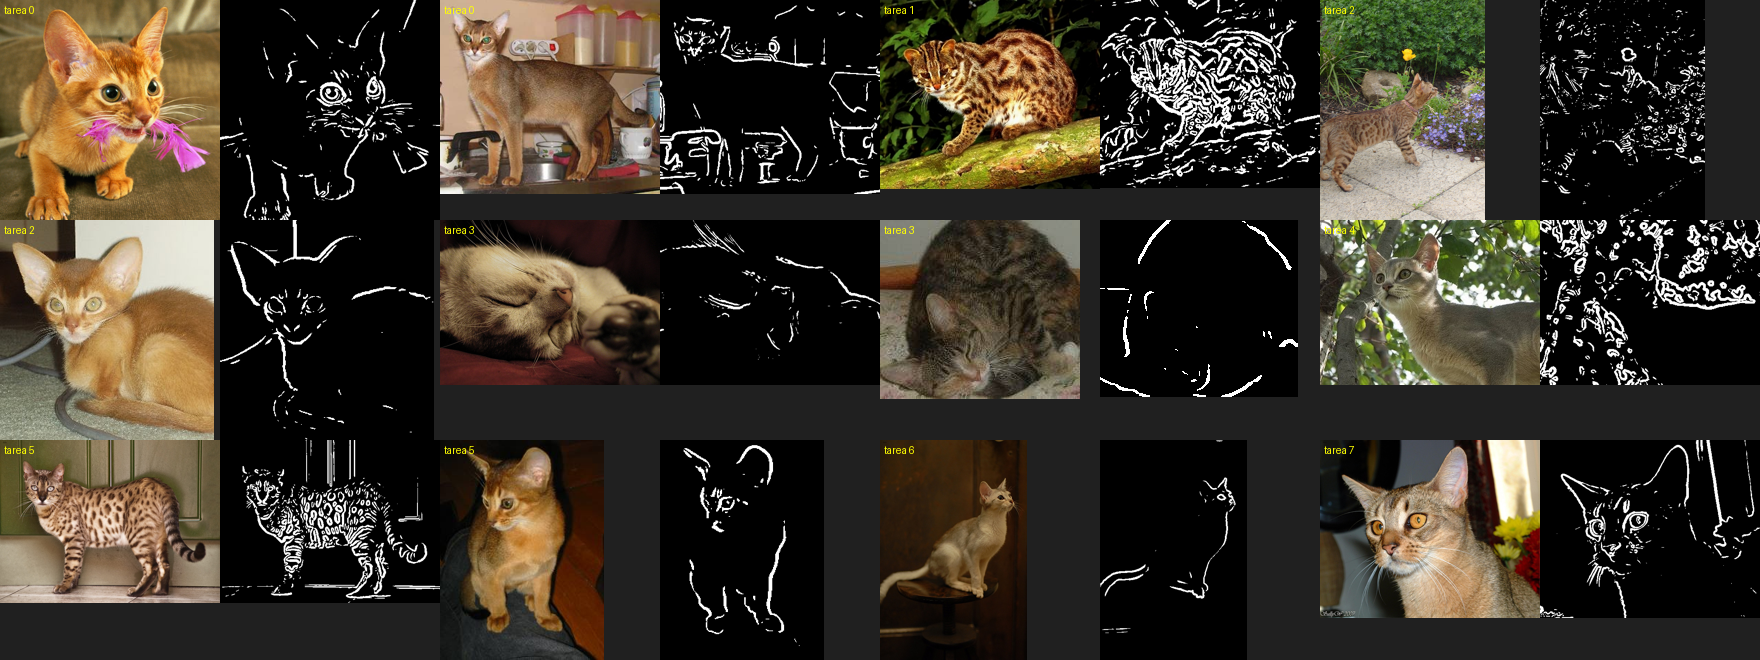
\includegraphics[width=0.8\linewidth]{demo/mosaico.png}
\caption{Corrida de demostración: 8 tareas, 4 en paralelo y 400 fotos. Cada par es la foto original y sus bordes, con la tarea que la procesó. \texttt{kubectl get pods -o wide} mostró los 8 índices repartidos en los 3 workers (4, 2 y 2), con 0 errores.}
\end{figure}

% ---------------------------------------------------------------- 2
\section{Resultados de rendimiento}

\begin{table}[H]
\centering
\small
\caption{Promedio de 3 repeticiones por combinación. La desviación estándar es de $T$. $I$ es el promedio de las 3 corridas.}
\begin{tabular}{@{}lrrrrrrr@{}}
\toprule
Estrategia & $p$ & $T(p)$ [s] & desv. [s] & $S(p)$ & $E(p)$ & $f$ & $I$\\
\midrule
block  & 1 & 140.0 &  9.5 & 1.00 & 1.00 & ---   & 1.256\\
block  & 2 &  74.3 & 12.9 & 1.88 & 0.94 & 0.062 & 1.277\\
block  & 4 &  39.7 &  0.6 & 3.53 & 0.88 & 0.044 & 1.210\\
block  & 8 &  34.0 &  3.6 & 4.12 & 0.51 & 0.135 & 1.136\\
\midrule
cyclic & 1 & 132.3 &  9.3 & 1.00 & 1.00 & ---   & 1.297\\
cyclic & 2 &  69.7 &  4.5 & 1.90 & 0.95 & 0.053 & 1.200\\
cyclic & 4 &  36.0 &  1.0 & 3.68 & 0.92 & 0.029 & 1.097\\
cyclic & 8 &  38.7 &  5.9 & 3.42 & 0.43 & 0.191 & 1.269\\
\midrule
lpt    & 1 & 130.0 &  6.1 & 1.00 & 1.00 & ---   & 1.341\\
lpt    & 2 &  66.3 &  3.8 & 1.96 & 0.98 & 0.021 & 1.194\\
lpt    & 4 &  37.0 &  2.6 & 3.51 & 0.88 & 0.046 & 1.142\\
lpt    & 8 &  37.3 &  8.1 & 3.48 & 0.44 & 0.185 & 1.147\\
\bottomrule
\end{tabular}
\end{table}

\begin{figure}[H]
\centering
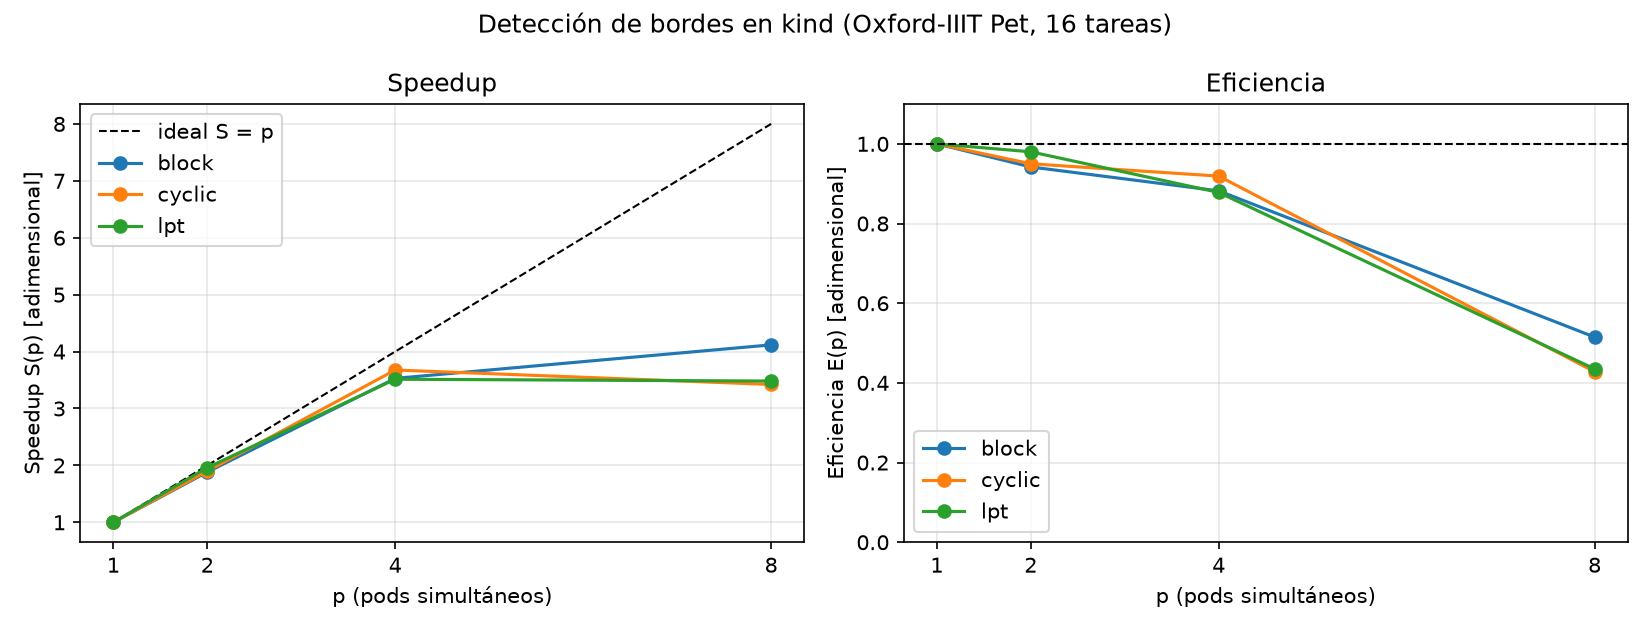
\includegraphics[width=\linewidth]{speedup.png}
\caption{Speedup y eficiencia por estrategia, con la recta ideal $S=p$.}
\end{figure}

\textbf{Hasta $p=4$ el escalamiento es casi lineal:} $S$ va de 3.5 a 3.7 y $E$ de 0.88 a 0.92. \textbf{De 4 a 8 ya casi no hay mejora.} block pasa de 3.53 a 4.12, y cyclic y lpt incluso bajan un poco; las diferencias entre estrategias con $p=8$ quedan dentro de la desviación, que es de 4 a 8~s. Medimos tres causas en \texttt{resultados/descomposicion.md}:

\begin{enumerate}
\item \textbf{Contención de CPU.} El promedio de ms por foto es 8.9 con $p=1$, 9.5 con $p=2$, 11.0 con $p=4$ y \textbf{24.5 con $p=8$}, 2.75 veces más lento. La laptop tiene 4 núcleos físicos: con 8 pods, dos comparten cada núcleo por hyper-threading, y además está corriendo el control-plane de kind. El límite de 1~CPU por pod no da núcleos que no existen. Pasamos de 4 a 8 pods, pero cada foto tarda 2.2 veces más que con $p=4$, así que la ganancia neta es casi nula.
\item \textbf{Arranque de pods.} Con $p=1$ los pods van uno tras otro y entre el fin de una tarea y el inicio de la siguiente pasan \textbf{4~s} (mediana de 135 huecos). Las 16 tareas suman 65.9~s de cómputo puro, pero $T(1)=134$~s: \textbf{51\,\% del tiempo es arrancar pods}, es decir, crear el pod, arrancar Python, importar numpy y Pillow y listar 7,390 archivos. Ese costo se reparte cuando hay más pods en paralelo, pero se paga 16 veces y con $p=8$ también compite por CPU.
\item \textbf{Disco compartido y cola de 16 tareas.} Los 8 pods leen del mismo SSD a través del \texttt{hostPath}. Además, con 16 tareas y $p=8$ hay solo 2 ``rondas'': si una tarea se retrasa, toda la ronda la espera.
\end{enumerate}

\textbf{Fracción serial.} Con $p=2$ y $p=4$, $f$ queda entre 0.02 y 0.06: según Amdahl, al menos el 94\,\% del trabajo es paralelizable. Con $p=8$, $f$ ``sube'' a 0.13--0.19. Esa subida no es código serial nuevo. Amdahl supone que la parte paralela se acelera $p$ veces, y aquí no pasa porque con más de 4 pods ya no hay núcleos libres. El $f$ estimado con $p=8$ mide en realidad la \textbf{saturación del hardware}, no un cuello de botella del programa.

% ---------------------------------------------------------------- 3
\section{Desbalance de carga}

\begin{figure}[H]
\centering
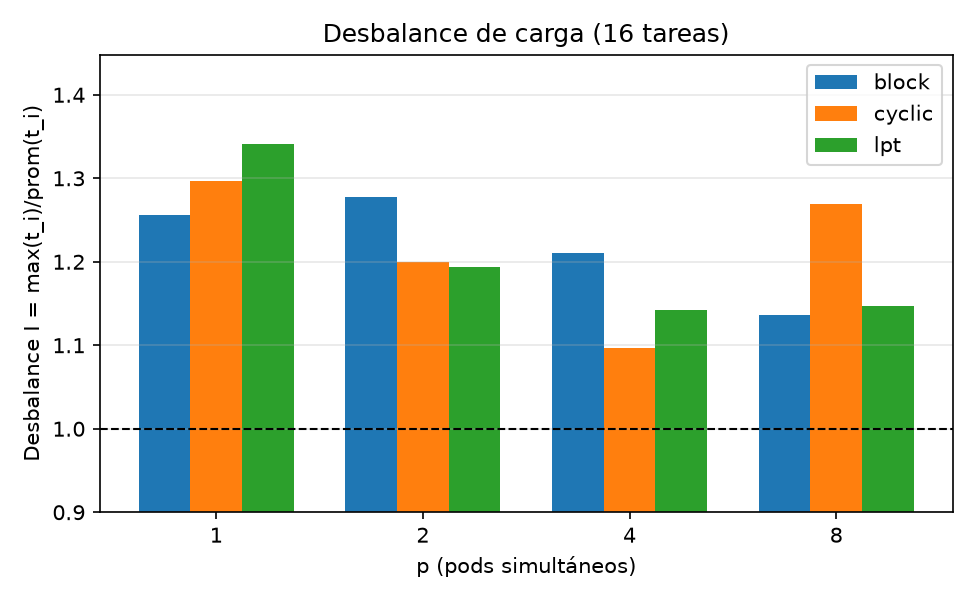
\includegraphics[width=0.49\linewidth]{desbalance.png}\hfill
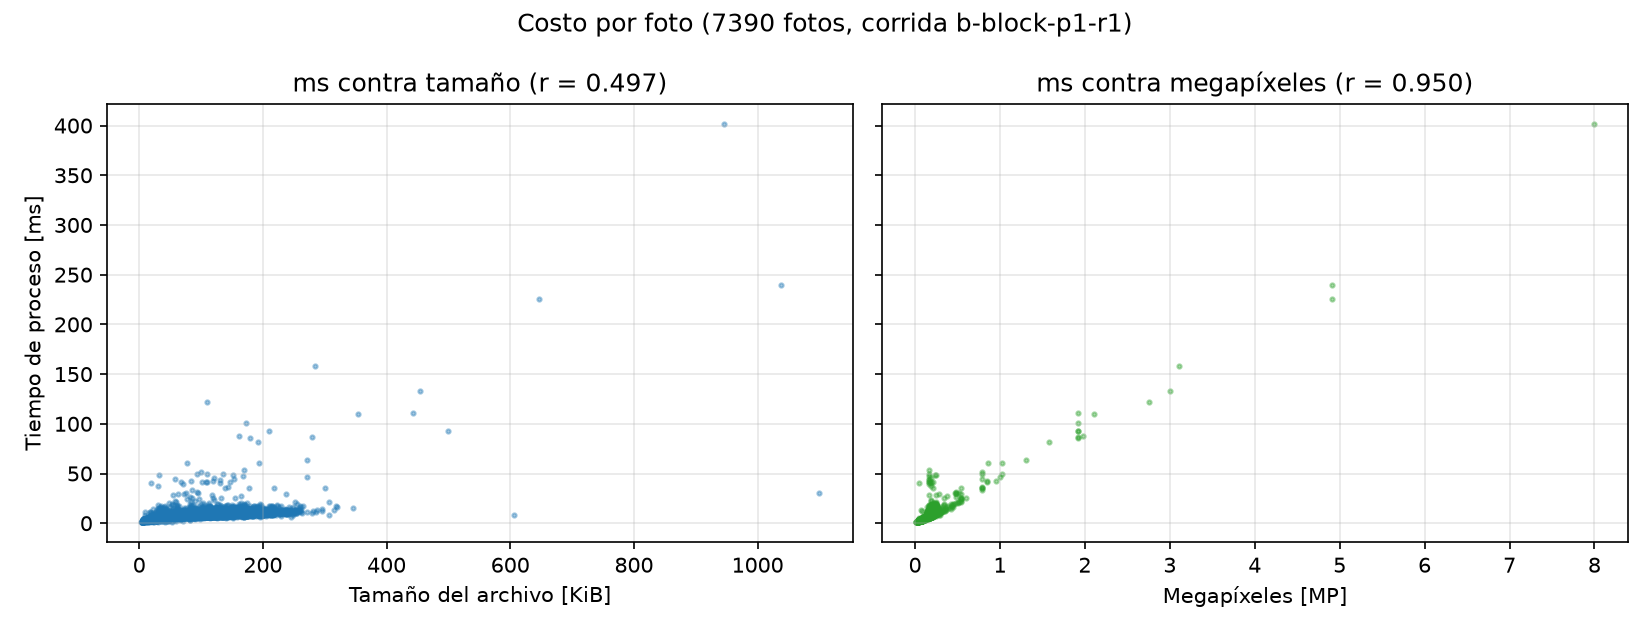
\includegraphics[width=0.49\linewidth]{costo_por_foto.png}
\caption{Izquierda: $I$ promedio por estrategia. Derecha: milisegundos por foto contra tamaño de archivo ($r = 0.50$) y contra megapíxeles ($r = 0.95$).}
\end{figure}

El $I$ medido tiene ruido. Por ejemplo, en la repetición 2 de lpt con $p=1$ una tarea tardó 7.7~s cuando las demás tardaron $\sim$3.8~s: coincidió con otro proceso usando la laptop. Por eso comparamos de dos formas:

\begin{itemize}
\item \textbf{Medido, mediana de 3 repeticiones, con $p=1$} (sin contención entre pods): block 1.185, cyclic 1.192 y \textbf{lpt 1.132}. Con $p>1$ las medianas cambian sin orden claro (de 1.09 a 1.29), porque el $t_i$ de cada tarea depende también de con quién compartió núcleo.
\item \textbf{Simulado con los ms reales de cada foto} (\texttt{descomponer.py}): block 1.185, cyclic 1.119 y \textbf{lpt por bytes 1.065}. Si LPT repartiera por megapíxeles sería 1.026, y la cota con los ms exactos es 1.000.
\end{itemize}

\textbf{lpt es el que mejor reparte.} Primero acomoda las fotos más caras y deja las pequeñas para emparejar al final. block es el peor porque la lista ordenada agrupa las razas: en la corrida \texttt{b-block-p1-r1}, el índice 10 recibió 54.5~MiB y tardó 4.98~s, y el índice 12 recibió 37.3~MiB y tardó 3.26~s, con las mismas 462 fotos. cyclic intercala razas y queda en medio. Aun así, \textbf{la estrategia casi no cambia $T(p)$}. Con 16 tareas de $\sim$4~s y un arranque de 4~s por pod, la diferencia entre la tarea más lenta y el promedio (menos de 1~s) pesa poco frente a la contención de CPU.

% ---------------------------------------------------------------- 4
\section{Tolerancia a fallos}

\texttt{scripts/prueba-fallo.sh} lanza 16 tareas con 4 en paralelo sobre 400 fotos y \texttt{FALLAR\_INDICE=3}. El worker del índice 3 deja una marca en el volumen compartido y sale con código 1. El reintento encuentra la marca y procesa normal. Evidencia en \texttt{resultados/fallo/}:
\begin{itemize}
\item \texttt{kubectl get pods}: el índice 3 tiene dos pods, \texttt{...-3-vwnlk} en \texttt{Error} y \texttt{...-3-6z56s} en \texttt{Completed}, los dos en \texttt{bordes-worker3}. Los otros 15 índices tienen un solo pod cada uno.
\item \texttt{kubectl describe job}: \texttt{Pods Statuses: 0 Active / 16 Succeeded / 1 Failed} y \texttt{Completed Indexes: 0-15}. En el estado, \texttt{failedIndexes} queda vacío y la condición es \texttt{Complete}.
\item Logs: \texttt{[3] Fallo provocado en el primer intento} y luego \texttt{[3] Reintento después del fallo provocado}, 25 fotos en 0.33~s.
\end{itemize}
Con \texttt{backoffLimitPerIndex}, el fallo se cuenta \textbf{por índice}: solo se repitió la tarea 3 y el Job terminó en 21~s. Con el \texttt{backoffLimit} global de antes, varios fallos en índices distintos se habrían sumado hasta tumbar todo el Job.

% ---------------------------------------------------------------- 5
\section{Preguntas de análisis}

\pregunta{Reparto}{¿Por qué repartir el mismo número de fotos a cada pod no garantiza que terminen al mismo tiempo?}{Porque el costo de una foto depende de sus píxeles, y los píxeles varían 570 veces entre la foto más chica (0.014~MP) y la más grande (8~MP). La más grande tardó 402~ms, contra una mediana de 8.9~ms: equivale a 45 fotos típicas. Con \texttt{block}, los 16 índices recibieron 461 o 462 fotos, pero sus tiempos fueron de 3.26~s (índice 12, 63.7~MP en total) a 4.98~s (índices 10 y 13, con 85.2 y 83.5~MP), con $I = 1.185$. Los índices más lentos fueron los que recibieron más megapíxeles: la tabla completa está en \texttt{resultados/detalle.md}.}

\pregunta{Costo}{¿El tamaño del archivo es un buen estimador del costo de procesar una foto?}{Solo regular. En las 7,390 fotos, la correlación entre ms y tamaño de archivo es $r = 0.50$, y entre ms y megapíxeles es $r = 0.95$. El pipeline trabaja sobre píxeles ya decodificados, y el tamaño del JPEG depende además de la compresión y de cuánto detalle tiene la escena. Por ejemplo, \texttt{Egyptian\_Mau\_14.jpg} pesa 1.1~MB pero tiene 0.47~MP y tardó 30~ms, mientras \texttt{Bombay\_140.jpg} pesa 110~KB, tiene 2.76~MP y tardó 122~ms. Por eso LPT por bytes deja $I = 1.065$ en la simulación y LPT por megapíxeles bajaría a 1.026. Los megapíxeles se leen del encabezado del JPEG sin decodificarlo, así que sería un cambio barato.}

\section*{Conclusiones}
El Job indexado reparte el lote sin coordinación entre pods: cada uno calcula su parte con su índice. En una laptop de 4 núcleos se llega a $S \approx 3.5$--$3.7$ con $p=4$, y \textbf{el límite lo pone el hardware}: con $p=8$ cada foto tarda 2.75 veces más. Arrancar pods cuesta el 51\,\% de $T(1)$; procesar más fotos por pod, o usar menos tareas más grandes, amortizaría ese costo. lpt reparte mejor que block, pero la estrategia de reparto pesa poco en $T(p)$ porque el desbalance (menos de 1~s) es chico frente a la contención de CPU. El examen repite el experimento en 3 laptops reales (carpeta \texttt{examen/}), con más núcleos pero con los datos por red.

\end{document}
